% das Papierformat zuerst
\documentclass[a4paper, 11pt]{article}
\usepackage[margin=3cm]{geometry}
\usepackage[utf8]{inputenc}
\usepackage[T1]{fontenc}
\usepackage[ngerman]{babel}
\usepackage{hyperref} % clickable refs
\usepackage{graphicx}
\usepackage[toc, numberedsection, style=altlist]{glossaries}
\usepackage{float}

\makeglossary
% Betreuer2: Produktname
% Betreuer2: Gls, s. seite
% Betreuer2: History bleibt erhalten
\title{Pflichtenheft}
\author{Kevin Birke \\ Felix Dörre \\ Fabian Hafner \\ Lucas Werkmeister \\ Dominic Ziegler \\ Anastasia Zinkina}
%\date{}

%Hack for referencing labels
\makeatletter
\def\namedlabel#1#2{\begingroup
    #2%
    \def\@currentlabel{#2}%
    \phantomsection\label{#1}\endgroup
}
\makeatother
% End: Hack for referencing labels

% Glossar: alle Einträge, aber ohne extra Referenzen
% http://tex.stackexchange.com/questions/115635/glossaries-suppress-pages-when-using-glsaddall
\newcommand*{\glsgobblenumber}[1]{}
\makeatletter
\newcommand*{\glsaddnp}[2][]{
  \glsdoifexists{#2}{
    \def\@glsnumberformat{glsgobblenumber}
    \edef\@gls@counter{\csname glo@#2@counter\endcsname}
    \setkeys{glossadd}{#1}
    \@gls@saveentrycounter
    \@do@wrglossary{#2}
  }
}
\newcommand{\glsaddallunused}[1][]{
  \edef\@glo@type{\@glo@types}
  \setkeys{glossadd}{#1}
  \forallglsentries[\@glo@type]{\@glo@entry}{
    \ifglsused{\@glo@entry}{}{
      \glsaddnp[#1]{\@glo@entry}}}
}
\makeatother

\renewcommand{\glsnamefont}[1]{\mdseries #1} % glossary entries shouldn’t be bold

% Glossar

% So sieht ein Glossar-Eintrag aus:
%
%\newglossaryentry{dijkstra}{
%  name={Dijkstra’s Algorithmus},
%  description={ein Algorithmus, um den optimalen Pfad in einem gerichteten Graphen zu finden}
%}
%\newglossaryentry{arc}{
%  name={Arc-Flags},
%  description={eine Technik, um Routenberechnung zu beschleunigen},
%  see={dijkstra}
%}
%
% Und so kann er im Dokument verwendet werden:
%
% lorem ipsum dolor sit \gls{arc}, consectetur
%
% End: Glossar

% usage: \counteditem{prefix}{refName} -> item '/prefixXX/' with label 'prefix:refName' (where XX is counted in increments of 10)
\makeatletter
\newcommand{\oitem}[2]{
  % define the counter
  \@ifundefined{c@oitem#1}{\newcounter{oitem#1}}{} % initialized at 0
  \addtocounter{oitem#1}{10}
  \item[\namedlabel{#1:#2}{/#1\arabic{oitem#1}/}]
}
\makeatother

% usage: \testfall{szenario}{ablauf}{ergebnis} oder \testfall[\ref{F:getesteteFunktion}]{szenario}{ablauf}{ergebnis}
\newcommand{\testfall}[4][]{
  \begin{description}
    \ifthenelse{\equal{#1}{}}
               {} % optional argument #1 is empty: skip
               {\item[Testet] #1}
    \item[Vorbedingungen] #2
    \item[Ablauf] #3
    \item[Erwartetes Ergebnis] #4
  \end{description}
}

% Betreuer: Rand reduzieren. (gemacht)
% Betreuer: Wichtig, viel Kriterien, GUI, Testfälle
% Betreuer: Präzise!!!
% hier beginnt das Dokument
\begin{document}
\shorthandoff{"}

% place a symbol before clickable links
% this has to come *after* \begin{document} because hyperref installs a \AtBeginDocument hook that updates the ref command.
\newcommand{\refsymbol}[0]{\scalebox{0.5}{$\nearrow$}}
\let\oldref\ref
\renewcommand{\ref}[1]{\refsymbol\oldref{#1}}
\let\oldgls\gls
\renewcommand{\gls}[1]{\refsymbol\oldgls{#1}}
\let\oldGls\Gls
\renewcommand{\Gls}[1]{\refsymbol\oldGls{#1}}
\let\oldglslink\glslink
\renewcommand{\glslink}[2]{\refsymbol\oldglslink{#1}{#2}}
\let\oldhyperref\hyperref
\renewcommand{\hyperref}[2][notActuallyOptional]{\refsymbol\oldhyperref[#1]{#2}}

\maketitle
\newpage
\tableofcontents
\newpage
% Betreuer: Berechnung von Punkt auf Kante zu Punkt auf Kante.  (KdBaum über Kanten) (gemackt)
% Betreuer: Profile exakt welcher Typ (gemacht)

% alle Glossareintraege
\newacronym[longplural=Personenkraftwagen]{pkw}{PKW}{Personenkraftwagen}
\newacronym[longplural=Lastkraftwagen]{lkw}{LKW}{Lastkraftwagen}
\newacronym{osm}{OSM}{OpenStreetMap}
\newacronym{gui}{GUI}{Graphical User Interface}
\newacronym[longplural={Points of interest}]{poi}{POI}{Point of interest}
\newacronym{gpx}{GPX}{GPS Exchange Format}

\newglossaryentry{profil}{
  name={Profil},
  description={Enthält für die Routenplanung relevante Informationen, z.B. die Höhe und das Gewicht des Fahrzeugs},
  plural={Profile}
}
\newglossaryentry{route}{
  name={Route},
  description={Ein Weg zwischen zwei Punkten auf je einem Wegstück}
}
\newglossaryentry{rendern}{
  name={rendern},
  description={Berechnung eines Bilds aus den zu rendernden Daten}
}
\newglossaryentry{schnellroute}{
  name={schnellste Route},
  description={die \gls{route} mit der geschätzt kürzesten Fahrzeit}
}
\newglossaryentry{wegbeschreibung}{
  name={Wegbeschreibung},
  description={Beschreibung einer \gls{route} durch eine Liste von Abbiegeanweisungen}
}
\newglossaryentry{arc}{
 name={Arc-Flags},
 description={eine Technik, um Routenberechnung zu beschleunigen}
}
\newglossaryentry{beschleunigung}{
 name={Beschleunigung},
 description={Ermöglicht eine schnellere Berechnung der angefragten Route},
 see={arc}
}
\newglossaryentry{kartendaten}{
  name={Kartendaten},
  description={Eine Datei im \gls{osm}-Format, die eine Karte in Form von Knoten, Kanten und Relationen mit weiteren Informationen enthält}
}
\newglossaryentry{standardprofil}{
  name={Standardprofil},
  description={Ein vorinstalliertes Profil für gängige \glspl{pkw} oder \glspl{lkw}},
  see={profil}  
}
\newglossaryentry{vorberechnung}{
  name={Vorberechnung},
  description={Wandelt die Kartendaten in ein effizienteres Format um und fügt auf dem Profil basierende Informationen hinzu, die eine schnelle Routenberechnung ermöglichen. Muss für jede neue \gls{kartendaten}/\gls{profil}-Kombination einmal ausgeführt werden}
}
\newglossaryentry{dezimalkoordinaten}{
  name={Dezimalkoordinaten},
  description={Ein Format für Geokoordinaten, nämlich:\\
  	``Breitengrad, Längengrad''\\
  	die jeweils der Form ``\texttt{[+-]?[0-9]+.[0-9]*}'' sind}
}
\newglossaryentry{history}{
  name={History},
  description={Speicherung von Anfragen für spätere Wiederverwendung}
}
% -------------------------------------------------------------- HIER BEGINNT DAS DOKUMENT WIRKLICH ---------------------------------
\section{Einleitung}
% Betreuer2: Vorberechnung dauert lange. "Expertenfeature"
% TODO history erwähnen
Das Produkt ist an Fahrer von Kraftfahrzeugen gerichtet; es soll ihnen die Planung einer Reise erleichtern, indem es ihnen die \gls{schnellroute} zwischen zwei angegebenen Punkten berechnet und anzeigt.

Dabei wird besonders darauf Wert gelegt, dass die berechnete Route mit dem benutzten Fahrzeug auch tatsächlich gefahren werden kann. Dazu werden verschiedene Beschränkungen (Abbiegeeinschränkungen, Tonnage- und Höhenbeschränkungen, Verbot für bestimmte Fahrzeugtypen) bei der Routenberechnung berücksichtigt. Für die Berechnung der Route soll eine Beschleunigungstechnik eingesetzt werden.

Das Produkt soll auf jedem handelsüblichen Desktop-Computer, wie ihn die Mehrheit der Zielgruppe besitzt, lauffähig sein. Die Kartendaten stammen aus dem \gls{osm}-Projekt.
%Lucas

% Betreuer: Abbiegungbeschränkung, "Route berechnen", (gemacht)
\section{Zielbestimmung}
%Lucas

\subsection{Musskriterien}
% Betreuer: Ausführlicher. (gemacht)
% Betreuer2: Thesen, was ist.
\begin{description}
\oitem{MK}{karteAnzeigen} Die Software soll die Karte auf dem Bildschirm anzeigen.
\oitem{MK}{karteRendern} Kartenkacheln \gls{rendern} (Nur Straßen ohne Namen) % nach fkt. Anforderungen verschieben?
\oitem{MK}{karteVerschieben} Der Benutzer kann die Kartenansicht verschieben.
\oitem{MK}{karteZoomen} Der Benutzer kann die Kartenansicht zoomen.
\oitem{MK}{startZielWaehlen} Der Benutzer kann Start- und Zielpunkt einer Route durch Mausklick auf der Karte auswählen.
\oitem{MK}{startZielZeigen} Der ausgewählte Start- und Zielpunkt wird auf der Karte angezeigt.
\oitem{MK}{routeBerechnen} Die Software soll die \gls{schnellroute} zwischen dem ausgewählten Start- und Zielpunkt berechnen.
\oitem{MK}{routeAnzeigen}  Die berechnete \gls{route} zwischen Start- und Zielpunkt wird auf der Karte angezeigt.
\end{description}

\subsection{Wunschkriterien}
\begin{description}
\oitem{WK}{beschlArc} Die Routenberechnung soll durch \gls{arc} beschleunigt werden.
\oitem{WK}{abbiegebeschraeung} Bei der Routenberechnung werden Abbiegeverbote aufgrund von Abbiegeeinschränkungen beachtet.
\oitem{WK}{einbahnstrasse} Bei der Routenberechnung werden Einbahnstraßen beachtet.
\oitem{WK}{fahrzeugtyp} Bei der Routenberechnung werden Durchfahrtsverbote für bestimmte Fahrzeugtypen beachtet.
\oitem{WK}{maximalgewicht} Bei der Routenberechnung werden Durchfahrtsverbote aufgrund des zulässigen Maximalgewichts und der Maximalhöhe/-breite des Fahrzeugs beachtet.
%\oitem{WK}{strassentyp}                                                                                                                   % TODO Welchen Straßentyp
\oitem{WK}{beschreibung} Für die berechnete \gls{route} soll eine \gls{wegbeschreibung} generiert werden.
\oitem{WK}{beschreibungExport} Die generierte \gls{wegbeschreibung} kann als HTML-Datei exportiert werden.
\oitem{WK}{history} Der Benutzer kann Berechnungsanfragen aus einer \gls{history} auswählen.
\oitem{WK}{routeExport} Die berechnete \gls{route} kann als GPX-Datei zur Benutzung in GPS-Geräten exportiert werden.
\oitem{WK}{fahrzeit} Bestimmung der Fahrzeit einer \gls{route} unter Berücksichtung vom Benutzer festgelegter Durchschnittsgeschwindigkeiten und der zulässigen Höchstgeschwindigkeiten der befahrenen Straßenabschnitte sowie von Wartezeiten an Ampeln.
\oitem{WK}{osmKacheln} Der Benutzer kann sich optional \gls{osm}-Kacheln anstelle der eigenen gerenderten Kacheln anzeigen lassen.
\oitem{WK}{profilerstellen} Der Benutzer kann ein \gls{profil} erstellen
\oitem{WK}{profilloeschen} Der Benutzer kann ein \gls{profil} löschen
\oitem{WK}{profilaendern} Der Benutzer kann ein \gls{profil} ändern
\oitem{WK}{profile} Zwischen mehreren \glslink{profil}{Profilen} wählen
\oitem{WK}{standardprofil} Es gibt ein \gls{standardprofil} für \glspl{pkw} und eins für \glspl{lkw} 
\oitem{WK}{koordinaten} Start- und Zielkoordinaten können auch als \gls{dezimalkoordinaten} angegeben werden.
\oitem{WK}{karteRendernStrassen} Straßennamen und Bezeichnungen in \ref{MK:karteRendern} einbeziehen.
\oitem{WK}{karteRendernOrtsnamen} Ortsnamen in \ref{MK:karteRendern} einbeziehen
\oitem{WK}{karteRendernDeko} Einbahnstraßen in \ref{MK:karteRendern} visualisieren
\oitem{WK}{karteRendernDeko2} Damit der Benutzer sieht dass das Programm nicht hängt  .... %TODO
\oitem{WK}{kartenKachelnPrefetch} Kacheln in der Umgebung des angezeigten Ausschnitts im Vorraus berechnen bzw. anfragen, obwohl sie nicht direkt sichtbar sind
% Betreuer: Profile(gemacht)

\end{description}

\subsection{Abgrenzungskriterien}
\begin{description}
\oitem{AK}{textSuche} Eine textuelle Suche nach Adressen oder \glspl{poi} ist nicht möglich.
\oitem{AK}{zwischenziele} Die Angabe von Zwischenzielen ist nicht möglich.
\oitem{AK}{standort} Eine Erkennung des aktuellen Standorts des Benutzers findet nicht statt.
\oitem{AK}{poi} Die Positionen von \glspl{poi} sowie Gebäude werden nicht auf der Karte angezeigt.
\oitem{AK}{verkehrszeichen} Ampeln und Verkehrszeichen werden nicht auf der Karte visualisiert.
\oitem{AK}{baustelle} Baustellen werden (über die in den Kartendaten enthaltenen Informationen hinaus) nicht berücksichtigt.
\oitem{AK}{stau} TMC-Verkehrsmeldungen zu Staus werden nicht berücksichtigt.
\oitem{AK}{fahrradFussBahn} Die Software ist kein Routenplaner für Fahrradfahrer, Fußgänger oder öffentliche Verkehrsmittel.
\oitem{AK}{altRoute} Alternativrouten können nicht berechnet werden.
\oitem{AK}{app} Die Software ist keine mobile Anwendung (App).
\oitem{AK}{webapp} Die Software ist keine Webanwendung.
\end{description}

\section{Produkteinsatz}
%Kevin

Das Produkt soll Autofahrern bei der Planung einer optimalen Fahrstrecke helfen.

\subsection{Anwendungsbereiche}
\begin{itemize}
\item Routenplanung
\end{itemize}

\subsection{Zielgruppe}
\begin{itemize}
\item Autofahrer
\item Beifahrer
\item Personen, welche Routen für diese zuteilen bzw. erstellen
\end{itemize}

\subsection{Betriebsbedingungen}
\begin{itemize}
\item Zu Hause
\item In Büroumgebungen
\end{itemize}

\section{Produktumgebung}
%Kevin

\subsection{Software}\label{subsec:Software}

\begin{itemize}
\item Betriebssystem: Linux, Windows, andere Betriebssysteme mit Java $\geq$ 7
\item Java-Laufzeitumgebung: Version 7 oder neuer
\end{itemize}

\subsection{Hardware}

\begin{itemize}
\item Ein Standard-PC mit angeschlossener Maus und Tastatur
\item Dieser sollte über einen Farbbildschirm mit der Auflösung von mindestens 1920$\times$1080 Pixeln verfügen
\item Es muss genügend Arbeitsspeicher (mindestens 4 Gigabyte) und Festplattenkapazität (mindestens 20 Gigabyte freier Speicher) vorhanden sein
\item Es muss die \hyperref[subsec:Software]{oben} genannte Software auf dem Computer lauffähig sein und bereits installiert und konfiguriert sein
\end{itemize}

\section{Funktionale Anforderungen}
% Betreuer: Weniger Text(gemacht)
% Felix
% Betreuer2: Profil wählen. (gemacht)
% Betreuer2: Ausfteilen Wusch/Muss. (gemacht)
% Betreuer2: Mehr punkeA
% Betreuer2: Maker anzeigen. (gemacht)
% Betreuer2: Vorberechnung Überschrift (gemacht)
% Betreuer2: Mit kriterien synchron
\subsection{Kernfunktionen}
\begin{description}
\oitem{F}{berechneNächstenPunktAufKante}
Bestimmung des nächsten Punkts auf einer Kante zu gegebenen Geokoordinaten
\oitem{F}{berechneRoute}
Berechnung der \glslink{schnellroute}{schnellsten Route} von einem Start- zu einem Zielpunkt auf dem Straßengraph
\oitem{F}{mercator}
Berechnung der Mercator-Projektion zu Geokoordinaten und umgekehrt
\oitem{F}{routeBeschleunigen}
Die \gls{arc} zur Routenberechnung benutzen (siehe \ref{F:berechneRoute}).
\oitem{WF}{gpxAusRoute}
Erzeugung einer GPX-Datei aus einer \gls{route}.
\oitem{WF}{saveHist}
Hinzufügen der letzen berechneten Route zur History.
\oitem{WF}{getHist}
Auswählen von Start- und Zielpunkt aus der History.
\end{description}

\subsection{Vorberechnung}
\begin{description}
\oitem{F}{routeBeschleunigenRechnen}
Berechnung der \gls{arc} für \ref{F:routeBeschleunigen}
\oitem{F}{routeBeschleunigenSpeichern}
Abspeichern der Ergebnisse aus \gls{vorberechnung} in eine Datei.
\oitem{F}{berechneAbstand}
Berechnen des realen Abstands (in km) zwischen 2 Geokoordinaten.
% Betreuer2: Bestimmen, Berechnen, nicht Stätzen (gemacht)
\oitem{F}{zeitSchaetzen}
Bestimmen der benötigten Zeit für ein Wegstück unter Berücksichtigung des \glslink{profil}{Profils}, der Ampeln, der Abbiegezeiten und des Straßentyps.
\oitem{F}{bestimmenFahrErlaubnis}
Bestimmen, ob ein Fahrzeug des aktuellen Profils einen Straßenabschnitt benutzen darf.
\oitem{WF}{routeBeschleunigenSpeichern}
Berechnung der \gls{arc} für \ref{F:routeBeschleunigen}
\end{description}

\subsection{Benutzerschnittstelle}
\begin{description}
\oitem{F}{startZielEingeben}
Start und Zielpunkt durch Mausklicks festlegen
\oitem{F}{berechneKachel}
Berechnen einer Bildkachel aus lokalen Kartendaten zu gegebener Detailstufe und gegebenem Ausschnitt.
\oitem{F}{bestimmeKantenInAusschnitt}
Bestimmen aller Kanten aus einem gegebenen Kartenausschnitt unter Berücksichtigung der Zoomstufe. (Benötigt für \ref{F:berechneKachel})
\oitem{F}{bestimmeKachelnInAusschnitt}
Bestimmen aller in einem Kartenausschnitt benötigten Kacheln.
\oitem{F}{zeichneKachel}
Darstellen von Kartenkacheln der entsprechenden Zoomstufe an der richtigen Stelle im \gls{gui}.
\oitem{F}{bestimmeKoordinatenAusPunkt}
Bestimmen der Geokoordinaten zu einem gegebenem Pixel auf der angezeigten Karte.
% Betreuer2: Aufteilen, Genauer TODO: sichherer Formulieren
\oitem{F}{ziehenZuAusschnitt}
Anwenden von einer Verschiebung der Karte auf den aktuellen Kartenausschnitt.
\oitem{F}{zoomenInZuAusschnitt}
Anwenden von einer Vergrößerung der Karte auf den aktuellen Kartenausschnitt.
\oitem{F}{zoomenOutZuAusschnitt}
Anwenden von einer Verkleinerung der Karte auf den aktuellen Kartenausschnitt.
\oitem{F}{zeigeRoute}
Anzeigen einer berechneten Route (\ref{F:berechneRoute}) auf den dargestellten Kacheln (\ref{F:zeichneKachel}). Beispiel in
Abbildung \ref{fig:mockupscreenshotmain}
\oitem{F}{zeigeStartZiel}
Anzeigen des aktuellen Start- und Zielpunkts. Beispiel in
Abbildung \ref{fig:mockupscreenshotmain}

% Betreuer2: 'Aufbauen' (gemacht)
\oitem{WF}{fetcheOnlineKachel}
Anfordern von bereits gerenderten Kacheln aus dem Internet.
\oitem{WF}{startZielGeo}
Start und Zielpunkt durch Eingabe von \gls{dezimalkoordinaten} festlegen
\oitem{WF}{bestimmeKachelnUmAusschnitt}
Bestimmen aller Kacheln um einen gegebenen Kartenausschnitt.
\oitem{WF}{bestimmeKachelnVorAusschnitt}
Bestimmen aller Kacheln in den naheliegenden Zoomstufen an den angezeigen Geokoordinaten. % TODO leicht holprig
\oitem{WF}{cacheKacheln}
Zwischspeichern berechneter Kacheln um neuberechnung zu vermeiden. % TODO ?
\end{description}

\subsection{Wegbeschreibung}
\begin{description}
\oitem{WF}{bestimmeAbbiegeAusRoute}
Bestimmung aller Abbiegevorgänge einer \gls{route}
\oitem{WF}{klassifiziereAbbiege}
Klassifizierung der Abbiegevorgänge (rechts, links, scharf rechts, scharf links, geradeaus, halblinks, halbrechts, halblinks, rechts halten, links halten, Nummer der Ausfahrt im Kreisverkehr)
\oitem{WF}{bestimmeAnweisungAusAbbiege}
Bestimmung einer textuellen Abbiegeanweisung aus einem Abbiegevorgang
\oitem{WF}{htmlAusBeschreibung}
Erzeugung einer HTML-Datei aus einer \gls{wegbeschreibung}
\end{description}

\subsection{Profilverwaltung}
\begin{description}
\oitem{WF}{neuesProfil} Anlegen eines neuen Profils
\oitem{WF}{loescheProfil} Löschen eines vorhandenen Profils
\oitem{WF}{aendereProfil} Ändern eines vorhandenen Profils
\oitem{WF}{waehleProfil} Auswahl eines aktuellen Profils
% Betreuer2: Answählen
\end{description}

\section{Produktdaten}
% Betreuer: Darstellung und Berechnung nur aus eigenen Daten. Steht noch nicht da.
%Anastasia
\subsection{Profildaten}
In einem \gls{profil} werden gespeichert:
\begin{description}
\oitem{D}{fahrzeugTyp}
Fahrzeugtyp (\gls{pkw}, \gls{lkw}, Bus, Motorrad)
\oitem{D}{hoehe}
Höhe des Fahrzeugs
\oitem{D}{breite}
Breite des Fahrzeugs
\oitem{D}{gewicht}
Gewicht des Fahrzeugs
\oitem{D}{geschwindigkeitAutobahn}
Durchschnittsgeschwindigkeit auf Autobahn/Schnellstraße
\oitem{D}{geschwindigkeitLandstrasse}
Durchschnittsgeschwindigkeit auf Landstraße
\end{description}

\subsection{Kartendaten}
Es werden gespeichert:
\begin{description}
\oitem{D}{osmDatei}
\gls{osm}-Dateien
\oitem{D}{vorberechnung}
Datei mit den Ergebnissen der \gls{vorberechnung}
\oitem{D}{renderingData}
Alle Daten die fürs \Gls{rendern} benötigt werden (siehe \ref{WK:karteRendernStrassen}, \ref{WK:karteRendernOrtsnamen}, \ref{WK:karteRendernDeko} und \ref{MK:karteRendern})

\end{description}

\subsection{Historydaten}
Für die History wird gespeichert:
\begin{description}
\oitem{D}{history}
Start- und Zielpunkt aus den vorherigen Anfragen des Benutzers
\end{description}
\section{Systemmodell}
% Betreuer2: Hierarchisch, Gesamt-App-Paket
\includegraphics[width=\linewidth]{Paketdiagramm}
\begin{description}
\oitem{PK}{program} Programm\\
Die Hauptsteuerklasse des Programms. Initialisiert die Anwendung.
\oitem{PK}{gui} GUI\\
Beinhaltet alle Komponenten des GUI außer \ref{PK:mapView}. Realisiert u.a \ref{MK:startZielWaehlen}.
\oitem{PK}{mapView} MapViewer\\
Das GUI Element, dass Kartenkacheln dynamisch renderen lässt, cachet und dann skaliert an der richtigen
Position im Fenster an. Realisiert u.a \ref{MK:karteAnzeigen}, \ref{MK:karteVerschieben}, \ref{MK:karteZoomen}, \ref{MK:startZielZeigen}, \ref{MK:routeAnzeigen}
\oitem{PK}{precalc} PreCalculator\\
Verarbeitet OSM Dateien in ein eigenes Format. Berechnet \gls{arc}. Erstellt eine platzoptimierte Darstellung des Graphen. Filtert nicht benutzte Daten aus der OSM.
\oitem{PK}{renderer} Renderer\\
Berechnet die Kacheln aus den vorbereiteten Daten. Realisiert \ref{MK:karteRendern}
\oitem{PK}{routeCalculator} RouteCalculator\\
Berechnet die Route aus den vorbereiteten Daten. Realisiert \ref{MK:routeBerechnen}
\oitem{PK}{fileIO} FileIO\\
Schreibt und lädt eigene Dateien in den zur Routenberechnung optimierten Dateiformaten.
\oitem{PK}{osmParser} OSMParser\\
Liest die OSM Karte (\ref{D:osmDatei}) und wandelt sie in eine, zur Vorberechnung benutzten Form im Hauptspeicher, um.
\end{description}
%Anastasia
\section{Nichtfunktionale Anforderungen und Qualitätsziele}

\begin{description}
\oitem{NF}{routeFuenfSek} \ref{F:berechneRoute} (Berechnung der Route) ist schneller als fünf Sekunden.
\oitem{NF}{knotenHalbeSek} \ref{F:berechneNächstenPunktAufKante} benötigt höchstens 500 ms.
\oitem{NF}{knotenWaysAnzahl} Die Software muss Daten mit mindestens x Knoten und y Ways verarbeiten können.
% Betreuer2: Noch mehr, rendern einer Kachel, Mausklicks
\end{description}
% Dominic

\section{Benutzeroberfläche}
% Betreuer: weniger Klicks? Startknopf.
% Betreuer: Elemente durchnummerieren. Einzeln erklären.
% Betreuer2: Favs, 
% Betreuer2: Links ziehen
% Betreuer2: Klicks wie belegen?
% Betreuer2: Reihenfolge Karte, Profil
\subsection{Hauptfenster}
\begin{figure}[H]
\centering
\includegraphics[width=0.7\linewidth]{mockup_screenshot_main}
\caption{Erster Entwurf}
\label{fig:mockupscreenshotmain}
\end{figure}
\begin{enumerate}
\item \glspl{profil}-Button: Starte Profilverwaltung, siehe Abbildung \ref{fig:mockupprofilverwaltung}
\item Karten-Button: Wähle eine Karte; falls für diese Karte-Profil-Kombination keine Vorberechnung vorhanden ist, siehe Abbildung \ref{fig:mockupscreenshotkeinevorberechnung}
\item ausgewählte Karte, ausgewähltes \gls{profil}
\item ausgewählter Startpunkt, ausgewähltes Ziel. Mit \ref{WK:koordinaten} ist hier auch Eingabe möglich, sonst nur Anzeige
\item \gls{wegbeschreibung}; falls sie nicht auf den Bildschirm passt, erscheint ein Scrollbalken
\item Karte (\ref{MK:karteAnzeigen})
\item Zoom-Buttons: ‘+’ zum Hereinzoomen, ‘-’ zum Herauszoomen
\item Rechtsklick-Kontextmenü: ‘Start hier‘ setzt den Startpunkt, ‘Ziel hier’ den Zielpunkt
\item Der ausgewählte Startpunkt
\item Der ausgewählte Zielpunkt
\item Die berechnete \gls{route}
\end{enumerate}

\subsection{Dialog: Keine Vorberechnung}
\begin{figure}[H]
\centering
\includegraphics[width=0.7\linewidth]{mockup_screenshot_nicht_berechnet}
\caption{Keine Vorberechnung}
\label{fig:mockupscreenshotkeinevorberechnung}
\end{figure}
\begin{enumerate}
\item Warnmeldung
\item ausgegraute Karte
\item \gls{vorberechnung}-Button
\end{enumerate}

\subsection{Dialog: Profilverwaltung}
% Lucas
\begin{figure}[H]
\centering
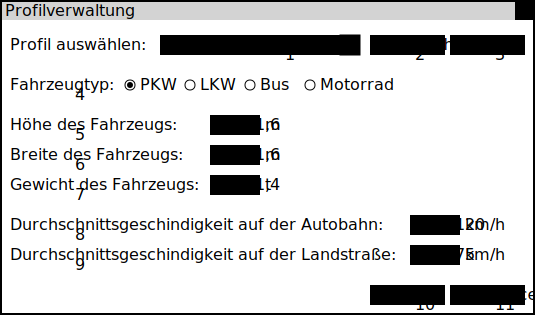
\includegraphics[width=0.7\linewidth]{Profilverwaltung}
\caption{Profilverwaltung}
\label{fig:mockupprofilverwaltung}
\end{figure}
% Betreuer2: Slider für die Zahl? Spinner?
\begin{enumerate}
\item Profil-Auswahl: Combobox (Dropdownmenü) zur Auswahl eines Profils
\item Löschen-Button: Löscht das aktuell ausgewählte Profil; bei Standardprofilen deaktiviert (\ref{WF:loescheProfil})
\item Neu-Button: Erstellt eine Kopie des aktuellen Profils; den Namen gibt der Benutzer in einem weiteren Dialog ein (\ref{WF:neuesProfil})
\item Fahrzeugtyp-Auswahl: Setzt den Fahrzeugtyp des aktuellen Profils (\ref{D:fahrzeugTyp})
\item Höhen-Eingabe: Setzt die Höhe des aktuellen Profils (\ref{D:hoehe})
\item Breiten-Eingabe: Setzt die Breite des aktuellen Profils (\ref{D:breite})
\item Gewicht-Eingabe: Setzt das Gewicht des aktuellen Profils (\ref{D:gewicht})
\item Autobahn-Geschwindigkeits-Eingabe: Setzt die Durchschnittsgeschwindigkeit des aktuellen Profils auf der Autobahn (\ref{D:geschwindigkeitAutobahn})
\item Landstraßen-Geschwindigkeits-Eingabe: Setzt die Durchschnittsgeschwindigkeit des aktuellen Profils auf der Landstraße (\ref{D:geschwindigkeitLandstrasse})
\item OK-Button: Speichert Änderungen am ausgewählten Profil, setzt es als das aktuelle Profil und schließt den Dialog
\item Abbrechen-Button: Verwirft Änderungen am ausgewählten Profil und schließt den Dialog
\end{enumerate}

\subsection{Dialog: Kartenauswahl}
\begin{figure}[H]
\centering
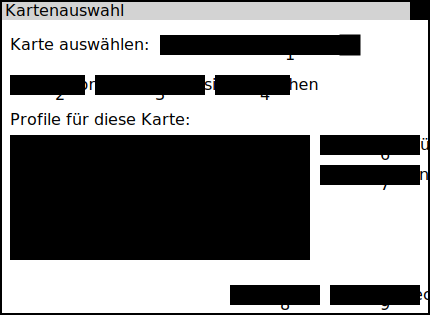
\includegraphics[width=0.7\linewidth]{Kartenauswahl}
\caption{Kartenauswahl}
\label{fig:mockupkartenauswahl}
\end{figure}
% TODO labeln
% Fabian

\section{Globale Testfälle und Szenarien}
% Betreuer: Vorbedinung, Aktionen, Nachbedingung
\subsection{Funktionssequenzen}
Bei allen Testfällen gilt als Vorbedingung, dass das Programm gestartet ist.
\begin{description}
\oitem{TF}{waehleErstenPunkt}\testfall
    {Karte ist sichtbar, Profil ist vorberechnet (für die aktuelle Karte)}
    {Auswählen des Start- bzw. Zielpunkts}
    {Start- bzw. Zielpunkt ist ausgewählt und wird auf der Karte angezeigt}
\oitem{TF}{waehleZweitenPunkt}\testfall
    [\ref{F:berechneRoute}, \ref{F:zeigeRoute}]
    {Karte ist sichtbar, Profil ist vorberechnet(für die aktuelle Karte),  Start- oder Zielpunkt ist ausgewählt (\ref{TF:waehleErstenPunkt})}
    {Auswählen des anderen Punkts (Ziel- bzw. Startpunkts)}
    {Route für die Angaben ist berechnet und wird angezeigt}
\oitem{TF}{waehlePunktErneut}\testfall
    [\ref{F:berechneRoute}, \ref{F:zeigeRoute}]
    {Karte ist sichtbar, Profil ist vorberechnet(für die aktuelle Karte),  Start- und Zielpunkt sind ausgewählt}
    {Erneutes Auswählen des  Ziel- oder Startpunkts}
    {Route für die neuen Angaben ist berechnet und wird angezeigt}
\oitem{TF}{zieheKarte}\testfall
    [\ref{F:zeichneKachel}, \ref{F:ziehenZuAusschnitt}]
    {Karte ist sichtbar}
    {Ziehen der Karte}
    {Die Kartenposititon hat sich entsprechend verändert}
\oitem{TF}{zoomeRein}\testfall
    [\ref{MK:karteZoomen}, \ref{F:zeichneKachel}]
    {Karte ist sichtbar}
    {Reinzoomen}
    {Ein Auschnitt der Karte wird größer und genauer dargestellt}
\oitem{TF}{zoomeRaus}\testfall
    [\ref{MK:karteZoomen}, \ref{F:zeichneKachel}]
    {Karte ist sichtbar}
    {Rauszoomen}
    {Ein größerer Bereich der Karte wird angezeigt}
\oitem{TF}{verbieteWaehlePunkt}\testfall
    {Karte ist sichtbar, aktuelles Profil ist nicht vorberechnet (für die aktuelle Karte)}
    {Versuchen Start- bzw. Zielpunkte auszuwählen}
    {Kein Start- oder Zielpunkt ist ausgewählt} % Betreuer2: Meldung, Popup nicht gut?, StatusBar
\oitem{TF}{starteVorberechnung}\testfall
    {Karte ist sichtbar, aktuelles Profil ist nicht vorberechnet (für die aktuelle Karte)}
    {Vorberechnung auswählen, lange Warten}
    {Aktuelles Profil ist vorberechnet (für die aktuelle Karte)}
\oitem{TF}{profilAnlegen}\testfall
    [\ref{WF:neuesProfil}]
    {Das erforderliche Profil ist noch nicht vorhanden}
    {Neues Profil anlegen}
    {Das neue Profil ist ausgewählt, das neue Profil ist nicht vorberechnet(für die aktuelle Karte)}
\oitem{TF}{waehleProfil}\testfall
    {Das erforderliche Profil ist vorhanden, aber nicht ausgewählt}
    {Ein Profil wird ausgewählt}
    {Das Profil ist ausgewählt}
\oitem{TF}{loescheProfil}\testfall
    [\ref{WF:loescheProfil}]
    {Ein Profil ist vorhanden}
    {Ein Profil wird gelöscht}
    {Das Profil ist nicht mehr vorhanden}
\oitem{TF}{importKarte}\testfall
    {Die Karte vorhanden}% Betreuer2: ganz weg
    {Eine neue Karte wird importiert}
    {Die neue Karte ist aktuell, kein Profil ist für die aktuelle Karte vorberechnet}
\oitem{TF}{waehleKarte}\testfall
    {Eine Karte ist ausgewählt}
    {Eine andere Karte wird ausgewählt}
    {Die andere Karte ist ausgewählt}
\oitem{TF}{speichereRoute}\testfall
    [\ref{WK:history}]
    {Eine Route ist berechnet}
    {Die Route wird gespeichert}
    {Die Route ist abgespeichert}
\oitem{TF}{ladeRoute}\testfall
    [\ref{WK:history}]
    {Eine Route ist abgespeichert}
    {Die abgespeicherte Route wird geladen}
    {Die abgespeicherte Route wird wieder angezeigt}
\oitem{TF}{standardProfil}\testfall
    {Ein \gls{standardprofil} existiert}
    {Versuchen das \gls{standardprofil} zu löschen}
    {Das \gls{standardprofil} ist nicht gelöscht}
\oitem{TF}{einbahnstrasse}\testfall
    {Karte ist sichtbar, Profil ist vorberechnet(für die aktuelle Karte), Karte enthält eine Einbahnstraße}
    {Als Startpunkt wird das Ende und als Ziel der Anfang der Einbahnstraße ausgewählt}
    {Ein Weg, der nicht diese Einbahnstraße beinhaltet, wird gefunden}
\oitem{TF}{geocoords}\testfall
    {Karte ist sichtbar, Profil ist vorberechnet (für die aktuelle Karte)}
    {Der Benutzer tippt Start- oder Zielkoordinaten als \gls{dezimalkoordinaten} ein}
    {Die Start- oder Zielkoordinaten sind nun auf die angegebenen abgeändert}
% Betreuer2: Wegbeschreibung export testen
% Betreuer2: Keine Interpretation
% Betreuer2: Systemstart
% Betreuer2: Gruppieren
% Betreuer2: Route anzeigen und Profil ändern
% Betreuer2: Mehr Beschränkungstests
% Betreuer2: kein beinhalten
% Betreuer2: Beenden und neu starten.

% Betreuer2: Karten/Kartendaten/Profil Begriff, Karte ^= Anschauen
% Betreuer2: Renderer ändern im GUI


% Betreuer2: Testszenarien
\end{description}
\subsection{Datenkonsistenzen}

\begin{description}
\oitem{TD}{datenProfilVorberechnung}
Eine Route kann nur berechnet werden, wenn \gls{kartendaten} vorliegen, ein \gls{profil} ausgewählt wurde und die \gls{vorberechnung} für dieses \gls{profil} für diese Karte abgeschlossen ist.
\oitem{TD}{gültigOsm}
\gls{kartendaten} müssen als gültige \gls{osm}-Datei vorliegen.
\oitem{TD}{karteProfilGelöscht}
Eine gespeicherte Route kann nicht angezeigt werden, wenn die zugehörigen Kartendaten und das verwendete \gls{profil} nicht mehr vorhanden sind.
\oitem{TD}{löscheNichtStandard}
Das \gls{standardprofil} kann nicht gelöscht werden.
\oitem{TD}{profil}
Es ist ein \gls{profil} ausgewählt.
\oitem{TD}{karte}
Es ist eine Karte ausgewählt.
\end{description}
% Fabian
\section{Entwicklungsumgebung}
\begin{description}
\item[Teamkommunikation] E-Mail-Verteiler, Skype
\item[Dokumentation] \LaTeX{}
\item[UML-Planungswerkzeug] UMLet
\item[IDE] Eclipse
\item[Qualitätssicherung] JUnit, CodeCover
\item[Versionskontrolle] Git
\end{description}
% Kevin

\glsaddallunused
\printglossary[type=main, title={Glossar}, toctitle={Glossar}]

\end{document}
